%%%%%%%%%%%%%%%%%%%%%%%%%%%%%%%%%%%%%%%%%%%%%%%%%%%%%%%%%%%%%%%%%%%%%%%%%%%%%%%%%%%%%%%%%%%%%%%%
%
% CSCI 1290 Written Question Template
%
% This is a LaTeX document. LaTeX is a markup language for producing documents.
% Your task is to answer the questions by filling out this document, then to 
% compile this into a PDF document. 
% You will then upload this PDF to `Gradescope' - the grading system that we will use. 
% Instructions for upload will follow soon.
%
% 
% TO COMPILE:
% > pdflatex thisfile.tex
%
% If you do not have LaTeX and need a LaTeX distribution:
% - Departmental machines have one installed.
% - Personal laptops (all common OS): http://www.latex-project.org/get/
%
% If you need help with LaTeX, come to office hours. Or, there is plenty of help online:
% https://en.wikibooks.org/wiki/LaTeX
%
% Good luck!
% James and the 1290 staff
%
%%%%%%%%%%%%%%%%%%%%%%%%%%%%%%%%%%%%%%%%%%%%%%%%%%%%%%%%%%%%%%%%%%%%%%%%%%%%%%%%%%%%%%%%%%%%%%%%
%
% How to include two graphics on the same line:
% 
% \includegraphics[width=0.49\linewidth]{yourgraphic1.png}
% \includegraphics[width=0.49\linewidth]{yourgraphic2.png}
%
% How to include equations:
%
% \begin{equation}
% y = mx+c
% \end{equation}
% 
%%%%%%%%%%%%%%%%%%%%%%%%%%%%%%%%%%%%%%%%%%%%%%%%%%%%%%%%%%%%%%%%%%%%%%%%%%%%%%%%%%%%%%%%%%%%%%%%

\documentclass[11pt]{article}

\usepackage[english]{babel}
\usepackage[utf8]{inputenc}
\usepackage[colorlinks = true,
            linkcolor = blue,
            urlcolor  = blue]{hyperref}
\usepackage[a4paper,margin=1.5in]{geometry}
\usepackage{stackengine,graphicx}
\usepackage{fancyhdr}
\setlength{\headheight}{15pt}
\usepackage{microtype}
\usepackage{times}

% From https://ctan.org/pkg/matlab-prettifier
\usepackage[numbered,framed]{matlab-prettifier}

\frenchspacing
\setlength{\parindent}{0cm} % Default is 15pt.
\setlength{\parskip}{0.3cm plus1mm minus1mm}

\pagestyle{fancy}
\fancyhf{}
\lhead{Project 1 Questions}
\rhead{CSCI 1290}
\rfoot{\thepage}

\date{}

\title{\vspace{-1cm}Project 1 Questions}


\begin{document}
\maketitle
\vspace{-3cm}
\thispagestyle{fancy}

\section*{Instructions}
\begin{itemize}
  \item 4 questions.
  \item Write code where appropriate.
  \item Feel free to include images or equations.
  \item Please make this document anonymous.
  \item \textbf{Please use only the space provided and keep the page breaks.} Please do not make new pages, nor remove pages. The document is a template to help grading.
  \item If you really need extra space, please use new pages at the end of the document and refer us to it in your answers.
\end{itemize}

\section*{Questions}

%%%%%%%%%%%%%%%%%%%%%%%%%%%%%%%%%%%

% Please leave the pagebreak
\paragraph{Q1a:} 
The following diagram shows the pinhole camera model. Rays emanating
from a an object pass through the pinhole $o$ and hit the image plane.

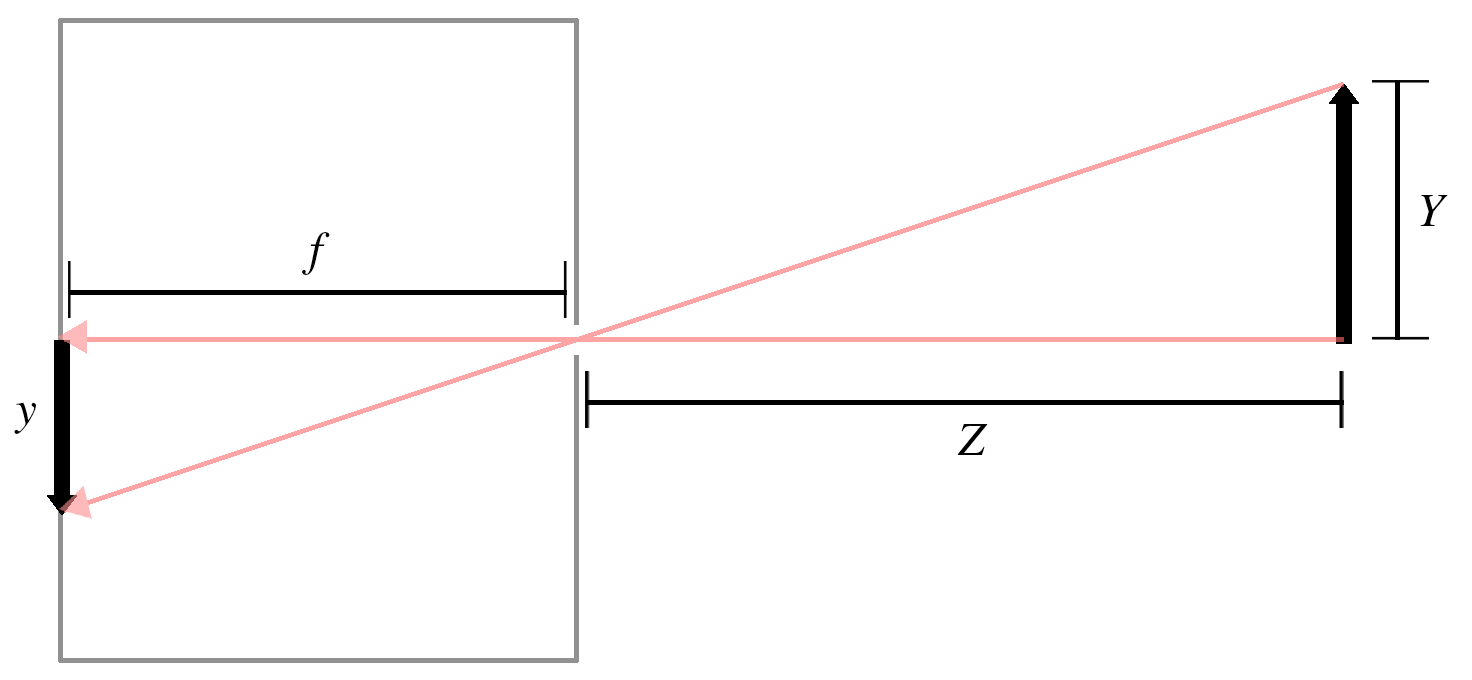
\includegraphics[width=0.8\linewidth]{pinhole.png}

What do the terms $f$, $Z$, $y$, and $Y$ represent?

\paragraph{A1a:} Your answer here.

\pagebreak
\paragraph{Q1b:}
Given $Y$, derive an equation for $y$ in terms of $Y$, $f$, and $D$.

\paragraph{A1b:} Your answer here.

\pagebreak
\paragraph{Q1c:}
The following diagram shows a thin lens model. Rays emanating from a point are refracted through the lens and converge at some point behind the lens. 

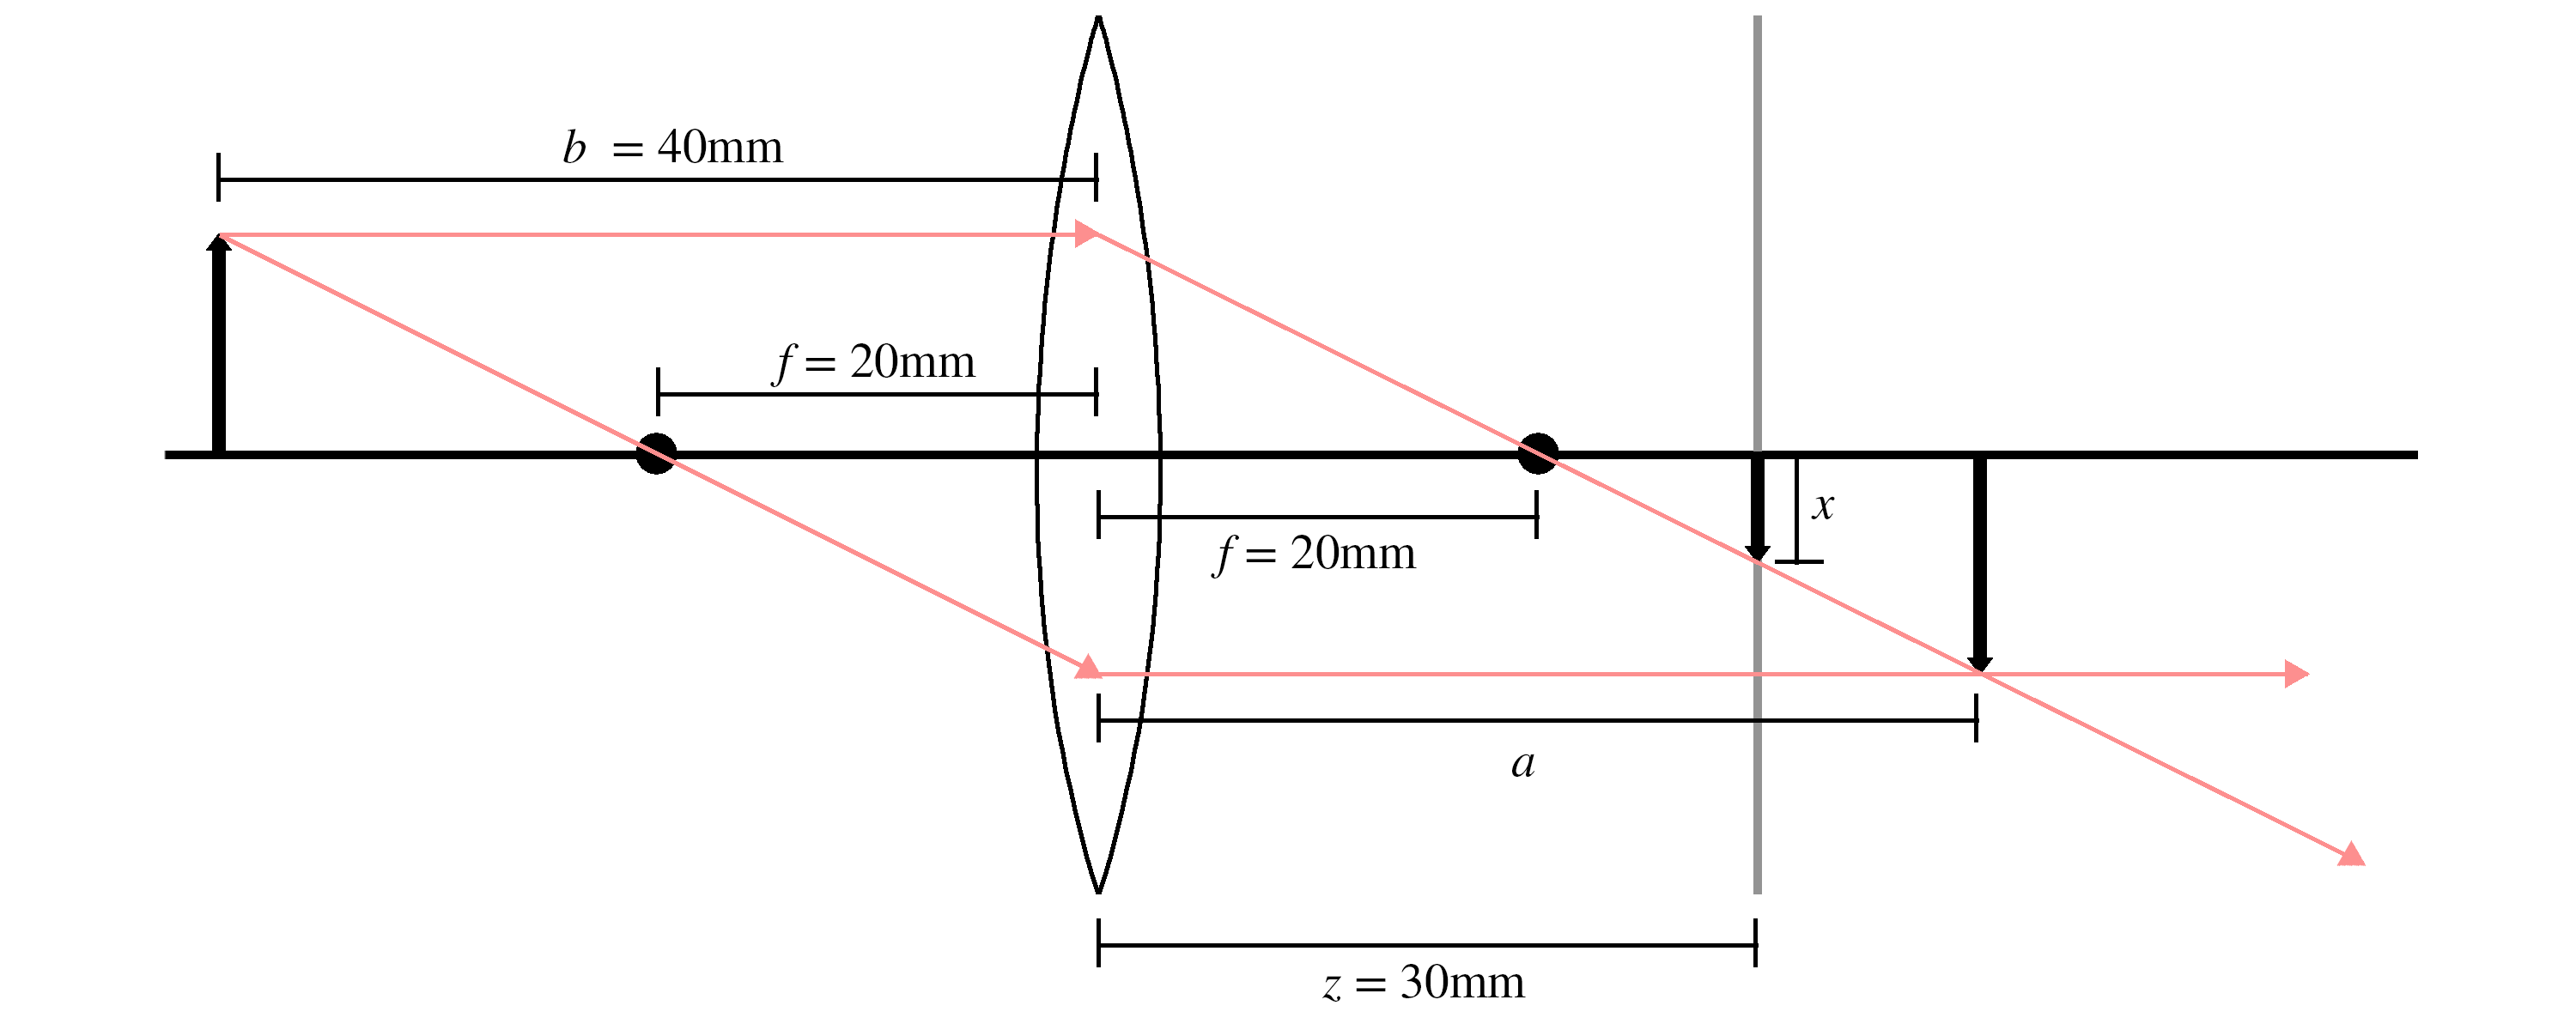
\includegraphics[width=1.0\linewidth]{lens.png}

The distance $a$ of the point at which the rays converge is determined by $b$, the distance of the object from the lens, and the focal length $f$ of the lens:

\begin{equation}
\frac{1}{a} = \frac{1}{f} - \frac{1}{b}
\end{equation}

The focal length $f$ of the camera is 20mm. If the image plane is located at a distance of $z =$ 30mm behind the lens, what is the size $x$ of the image of a scene point located at distance of $b = $40mm from the lens? 

%%%%%%%%%%%%%%%%%%%%%%%%%%%%%%%%%%%
\paragraph{A1c:} Your answer here.


%%%%%%%%%%%%%%%%%%%%%%%%%%%%%%%%%%%
\pagebreak
\paragraph{Q2:} 

Describe the relationship between shutter speed, ISO, and the aperture size of a camera. How does each relate to both the exposure of the image and the noise in the image? Feel free to use equations or graphs to help explain these concepts.

%%%%%%%%%%%%%%%%%%%%%%%%%%%%%%%%%%%
\paragraph{A2:} Your answer here.


%%%%%%%%%%%%%%%%%%%%%%%%%%%%%%%%%%%

% Please leave the pagebreak
\pagebreak
\paragraph{Q3:} 
Take a noisy photo (in low light conditions or by using manual controls, for instance), and use your knowledge of filtering to denoise it. Why did you pick this strategy, and what are the pros and cons of your approach?

Include the original image, the filtered image, and your MATLAB code.

%%%%%%%%%%%%%%%%%%%%%%%%%%%%%%%%%%%
\paragraph{A3:} Your answer here.



%%%%%%%%%%%%%%%%%%%%%%%%%%%%%%%%%%%

% Please leave the pagebreak
\pagebreak
\paragraph{Q4:} 

Using what you have learned so far about digital cameras, imaging, and sampling, take an \emph{interesting photo} (intentionally vague!). Image manipulation is allowed; cited inspiration is also welcomed! 

We will share the images with the class in the next lab.

%%%%%%%%%%%%%%%%%%%%%%%%%%%%%%%%%%%
\paragraph{A4:} Your answer here.



%%%%%%%%%%%%%%%%%%%%%%%%%%%%%%%%%%%


% If you really need extra space, uncomment here and use extra pages after the last question.
% Please refer here in your original answer. Thanks!
%\pagebreak
%\paragraph{AX.X Continued:} Your answer continued here.



\end{document}
